\documentclass{report}
\usepackage[T1]{fontenc}
\usepackage[margin=0.75in]{geometry}
\usepackage[bottom]{footmisc}
\usepackage{float}
\usepackage{placeins}
\usepackage{booktabs}
\usepackage{xcolor}
\usepackage{listings}
\usepackage{url}
\usepackage{graphicx}
\usepackage{verbatim}
\usepackage{ftnxtra}
\usepackage{fnpos}
\usepackage{caption}
\usepackage{subcaption}
\usepackage{amsmath}
\usepackage{afterpage}

\usepackage{hyperref}
\hypersetup{
    colorlinks,
    citecolor=blue,
    filecolor=blue,
    linkcolor=blue,
    urlcolor=blue
}

% ------------------------------------
% New Environment commands
% ------------------------------------

\newcommand\blankpage{%
    \null
    \thispagestyle{empty}%
    \addtocounter{page}{-1}%
    \newpage}

% ------------------------------------
% Start Document
% ------------------------------------

\title{Learning Idioms and Slang using a Deep Learning approach with Speech Recognition}
\author{Davide Berdin \\
  \texttt{ \{davide.berdin.0110\}@student.uu.se} \\
  \\ Master Thesis
  \\ Department of Information Technology}

\begin{document}

\maketitle

% Dedication
\blankpage
\thispagestyle{empty}
    \null\vspace{\stretch {1}}
        \begin{flushright}
                \begin{em}
                    To my family that never stopped believing in me
                \end{em}
        \end{flushright}
\vspace{\stretch{2}}

\blankpage

\tableofcontents{}

\begin{abstract}
Lorem ipsum dolor sit amet, consectetur adipiscing elit, sed do eiusmod tempor incididunt ut labore et dolore magna aliqua. Ut enim ad minim veniam, quis nostrud exercitation ullamco laboris nisi ut aliquip ex ea commodo consequat. Duis aute irure dolor in reprehenderit in voluptate velit esse cillum dolore eu fugiat nulla pariatur. Excepteur sint occaecat cupidatat non proident, sunt in culpa qui officia deserunt mollit anim id est laborum.
\end{abstract}

%%%%%% Chapters %%%%%%

\chapter{Introduction}
The pronunciation is one of the hardest part of learning a language among all the other components, such as grammar rules and vocabulary. To achieve a good level of pronunciation, non native speakers have to study and constantly practice the target language for a incredible amount of hours. In most cases, when students are learning a new language, the teacher is not a native speaker in which implies that the pronunciation may be influenced by the country where he or she comes from, since it is a normal consequence of second learning language \cite{derwing2005second}. In fact, \cite{medgyes2001teacher} states that the advantages of having a native speaker as a teacher, lies in the superior linguistic competences, especially the usage of the language more spontaneously in different communication situations. Pronunciation falls into those competences underlying a base problem in teaching pronunciation at school. \\

\noindent The basic questions we tried to answer in this work are:
\begin{compactitem}
    \item[1)] Why is pronunciation so important?
    \item[2)] What are the most effective methods for improving the pronunciation?
    \item[3)] What is the research state-of-art and what can we do to make it better?
\end{compactitem}

\vspace*{1em}

\noindent The first question is fairly easy to answer. There are two reasons to claim why pronunciation is important: \textit{(i)} it helps to acquire the target language faster and \textit{(ii)} being understood.
Regarding the first point, earlier a learner masters the basics of pronunciation, the faster it will become fluent. The reason is because \textit{critical listening} with a particular focus on hearing the sounds will lead to gain fluency in speaking the language.
The second point is \textbf{crucial} when working with other people, especially at these days where both in school and business the environment is often multicultural. Pronunciation mistakes may lead the person to being misunderstood affecting the results of a project for example. \\

\noindent With these statements in mind, \cite{gilakjani2011pronunciation} gives suggestions on how a learner can effectively improve the pronunciation. Four important ways are depicted: \textit{Conversation} is the most relevant approach to improve pronunciation, although, a supervision of an \textit{expert guidance} that corrects the mistakes is fundamental during the process of learning. At the same time, learners have to be pro-active to have conversation with other native speakers in such a way to constantly practicing. \textit{Repetitions} of pronunciation exercises is another important factor that will help the learner to be better in speaking. As last, \textit{Critical listening}, that we also mentioned above, amplify the opportunity of learning the way native speakers pronounce words. In particular, for a learner is important to understand the difference when he or she is pronouncing a certain sentence with the one said by the native speaker. This method is very effective and is important for understanding the different sounds of the language and how a native speaker is able to reproduce them \cite{rost2014listening}.

\noindent An important factor while learning a second language is to have a feedback about improvements. Teachers are usually responsible to judge the way the learners' progress. In fact, when teaching pronunciation, often it is used to draw the intonation and the stress of the words in such a way that the learner is able to see how the utterances should be pronounced. The \textit{British Council} shows this practice \cite{bbc_stress}. The usage of visual feedbacks is the key of learning pronunciation and it is the main feature of this research. \\

\noindent In the computer science field, some works have been previously done regarding pronunciation. For instance, \cite{edge2012tip} helps learners to acquire the tonal sound system of Mandarin Chinese through a mobile game. Another example is \cite{head2014tonewars} in which the application provides a platform where learners of Chinese language can interact with native speakers and challenging them to a competition of pronunciations of Chinese tones. \\

\noindent The idea behind this project is based on the fact that people need to keep practicing their pronunciation to have a significant improvement as well as they need immediate feedbacks to understand if they are going in the right direction or not. The approach we used is based on these two factors and we designed the system to be as useful and portable as possible. The mobile application is where the user will test the pronunciation, a server through a machine learning technique will compute the similarity between the user's pronunciation and the native speaker's one and the results will be displayed on the phone. \\

\noindent We started collecting data from \textit{American Native Speakers} in which we asked to pronounced a set of most used idioms and slangs. Each candidate had to repeat the same sentence several times trying to be as consistent as possible. After we gathered the data, a preprocessing step is due since we are seeking for specific features such as voice-stress, accent, intonation and formants. 
This part has been done using an external tool called \textbf{FAVE-Extract} in which it uses \textbf{PRAAT}\cite{boersma2010p} to analyze the sound. At this point, the next step is processed differently when treating native speaker files because we use manually defined the correct \textit{phonemes} for each sentence. This step is called \textbf{force alignment} in which it is estimated the beginning and the end of when a phoneme is pronounced by the speaker. For non-native speakers we used the phonemes that we extracted using the speech recognition system. \\

\noindent The machine learning part is divided in two: the first consists in using the library called \textbf{CMU Sphinx 4} with an acoustic model trained with all the data we collected from the native speakers. This library is a \textbf{HMM-based} system with multiple searching systems written in Java. To estimate the overall error between the native pronunciation and the user, we use a method called \textbf{Word Error Rate} (WER), a common method metric for measuring the performance of a speech recognition system. 
The second part consists in using a \textbf{Gaussian Mixture Model} (GMM) that we used to predict the vowels pronounced by the user. The result should help the user to better understand \textit{how close} is his/her vowels pronunciation compared with the native ones. \\

\noindent After the server has computed the speech recognition extracting the phonemes and predicted the similarity of vowels, the system creates graphs that will be used in the mobile application as feedback. In this way the user has a clear understanding of how he/she should \textbf{adjust} the way the utterance have to be pronounced. \\

\noindent To measure the accuracy of our model, we asked 10 native speakers to rate the pronunciation of 10 non native speakers on 5 different sentences. The range of evaluation was between 0 and 10. From here we averaged all the rates and compared with the results obtained by the automatic system.

\chapter{Artificial Neural Networks}
\section{Artificial Neuron}
Our brain is composed by biological neurons and an artificial neuron (or AN) is a representation of it. Every AN can gather signals from other nurons or from the environment, and after an elaboration it transmits another signal to all the other ANs that are connected to it \cite{engelbrecht2007computational}. A rapresentation of AN is depicted in \ref{fig:artificial_neuron}. \\
Each connection to the artificial neuron has a numerical weigth associated to it in which the input signal is hold back. The value of the weight can be either positive or negative. In most cases, the sums of each node are weighted and then given as input to a \textit{non-linear} function called \textbf{transfer function} or \textbf{activation function} \cite{artificial_neuron_wiki}.

\begin{figure}[!ht]
    \centering
    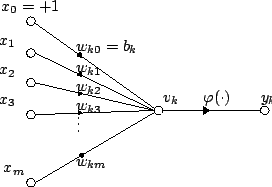
\includegraphics[scale=0.5]{Figures/artificial_neuron.png}
    \caption{Representation of an Artificial Neuron \cite{artificial_neuron_wiki}}
    \label{fig:artificial_neuron}
\end{figure}

\noindent From the mathematical point of view, we can define an artificial neuron as follow: \\
given $m+1$ inputs with signals from $x_1$ to $x_m$ and weights values from $w_0$ to $w_m$. The \textit{bias} is then defined by the input $x_0$ in which a value of 1 will be assigned. The bias value allows us to \textit{shift} the curve of the activation function to a certain direction and it is defined with $w_{k0} = b_k$ \cite{artificial_neuron_wiki}. \\
The output of the AN is:

\begin{equation*}
    y_k = \varphi \left ( \sum_{j=0}^{m} w_{kj} x_j \right )
\end{equation*}

\section{Network Function}
The word network in the term "artificial neural network" refers to the interconnections between the neurons in the different layers of each system. An example system has three layers. The first layer has input neurons which send data via synapses to the second layer of neurons, and then via more synapses to the third layer of output neurons. More complex systems will have more layers of neurons, some having increased layers of input neurons and output neurons. The synapses store parameters called "weights" that manipulate the data in the calculations.

\section{Learning}
Lorem ipsum dolor sit amet, consectetur adipiscing elit, sed do eiusmod tempor incididunt ut labore et dolore magna aliqua. Ut enim ad minim veniam, quis nostrud exercitation ullamco laboris nisi ut aliquip ex ea commodo consequat. Duis aute irure dolor in reprehenderit in voluptate velit esse cillum dolore eu fugiat nulla pariatur. Excepteur sint occaecat cupidatat non proident, sunt in culpa qui officia deserunt mollit anim id est laborum. \\

\subsection{Supervised Learning}
Lorem ipsum dolor sit amet, consectetur adipiscing elit, sed do eiusmod tempor incididunt ut labore et dolore magna aliqua. Ut enim ad minim veniam, quis nostrud exercitation ullamco laboris nisi ut aliquip ex ea commodo consequat. Duis aute irure dolor in reprehenderit in voluptate velit esse cillum dolore eu fugiat nulla pariatur. Excepteur sint occaecat cupidatat non proident, sunt in culpa qui officia deserunt mollit anim id est laborum. \\

\subsection{Unsupervised Learning}
Lorem ipsum dolor sit amet, consectetur adipiscing elit, sed do eiusmod tempor incididunt ut labore et dolore magna aliqua. Ut enim ad minim veniam, quis nostrud exercitation ullamco laboris nisi ut aliquip ex ea commodo consequat. Duis aute irure dolor in reprehenderit in voluptate velit esse cillum dolore eu fugiat nulla pariatur. Excepteur sint occaecat cupidatat non proident, sunt in culpa qui officia deserunt mollit anim id est laborum. \\

\subsection{Reinforcement Learning}
Lorem ipsum dolor sit amet, consectetur adipiscing elit, sed do eiusmod tempor incididunt ut labore et dolore magna aliqua. Ut enim ad minim veniam, quis nostrud exercitation ullamco laboris nisi ut aliquip ex ea commodo consequat. Duis aute irure dolor in reprehenderit in voluptate velit esse cillum dolore eu fugiat nulla pariatur. Excepteur sint occaecat cupidatat non proident, sunt in culpa qui officia deserunt mollit anim id est laborum. \\

\section{Multilayer Perceptron}
Lorem ipsum dolor sit amet, consectetur adipiscing elit, sed do eiusmod tempor incididunt ut labore et dolore magna aliqua. Ut enim ad minim veniam, quis nostrud exercitation ullamco laboris nisi ut aliquip ex ea commodo consequat. Duis aute irure dolor in reprehenderit in voluptate velit esse cillum dolore eu fugiat nulla pariatur. Excepteur sint occaecat cupidatat non proident, sunt in culpa qui officia deserunt mollit anim id est laborum. \\

\subsection{Activation Function}
Lorem ipsum dolor sit amet, consectetur adipiscing elit, sed do eiusmod tempor incididunt ut labore et dolore magna aliqua. Ut enim ad minim veniam, quis nostrud exercitation ullamco laboris nisi ut aliquip ex ea commodo consequat. Duis aute irure dolor in reprehenderit in voluptate velit esse cillum dolore eu fugiat nulla pariatur. Excepteur sint occaecat cupidatat non proident, sunt in culpa qui officia deserunt mollit anim id est laborum. \\

\subsection{Layers}
Lorem ipsum dolor sit amet, consectetur adipiscing elit, sed do eiusmod tempor incididunt ut labore et dolore magna aliqua. Ut enim ad minim veniam, quis nostrud exercitation ullamco laboris nisi ut aliquip ex ea commodo consequat. Duis aute irure dolor in reprehenderit in voluptate velit esse cillum dolore eu fugiat nulla pariatur. Excepteur sint occaecat cupidatat non proident, sunt in culpa qui officia deserunt mollit anim id est laborum. \\

\subsection{Learning through Backpropagation}
Lorem ipsum dolor sit amet, consectetur adipiscing elit, sed do eiusmod tempor incididunt ut labore et dolore magna aliqua. Ut enim ad minim veniam, quis nostrud exercitation ullamco laboris nisi ut aliquip ex ea commodo consequat. Duis aute irure dolor in reprehenderit in voluptate velit esse cillum dolore eu fugiat nulla pariatur. Excepteur sint occaecat cupidatat non proident, sunt in culpa qui officia deserunt mollit anim id est laborum. \\

\subsubsection{Gradient Descent}
Lorem ipsum dolor sit amet, consectetur adipiscing elit, sed do eiusmod tempor incididunt ut labore et dolore magna aliqua. Ut enim ad minim veniam, quis nostrud exercitation ullamco laboris nisi ut aliquip ex ea commodo consequat. Duis aute irure dolor in reprehenderit in voluptate velit esse cillum dolore eu fugiat nulla pariatur. Excepteur sint occaecat cupidatat non proident, sunt in culpa qui officia deserunt mollit anim id est laborum. \\

\chapter{Continuing with the journey...}
Lorem ipsum dolor sit amet, consectetur adipiscing elit, sed do eiusmod tempor incididunt ut labore et dolore magna aliqua. Ut enim ad minim veniam, quis nostrud exercitation ullamco laboris nisi ut aliquip ex ea commodo consequat. Duis aute irure dolor in reprehenderit in voluptate velit esse cillum dolore eu fugiat nulla pariatur. Excepteur sint occaecat cupidatat non proident, sunt in culpa qui officia deserunt mollit anim id est laborum. \\

Lorem ipsum dolor sit amet, consectetur adipiscing elit, sed do eiusmod tempor incididunt ut labore et dolore magna aliqua. Ut enim ad minim veniam, quis nostrud exercitation ullamco laboris nisi ut aliquip ex ea commodo consequat. Duis aute irure dolor in reprehenderit in voluptate velit esse cillum dolore eu fugiat nulla pariatur. Excepteur sint occaecat cupidatat non proident, sunt in culpa qui officia deserunt mollit anim id est laborum. \\

Lorem ipsum dolor sit amet, consectetur adipiscing elit, sed do eiusmod tempor incididunt ut labore et dolore magna aliqua. Ut enim ad minim veniam, quis nostrud exercitation ullamco laboris nisi ut aliquip ex ea commodo consequat. Duis aute irure dolor in reprehenderit in voluptate velit esse cillum dolore eu fugiat nulla pariatur. Excepteur sint occaecat cupidatat non proident, sunt in culpa qui officia deserunt mollit anim id est laborum. \\

Lorem ipsum dolor sit amet, consectetur adipiscing elit, sed do eiusmod tempor incididunt ut labore et dolore magna aliqua. Ut enim ad minim veniam, quis nostrud exercitation ullamco laboris nisi ut aliquip ex ea commodo consequat. Duis aute irure dolor in reprehenderit in voluptate velit esse cillum dolore eu fugiat nulla pariatur. Excepteur sint occaecat cupidatat non proident, sunt in culpa qui officia deserunt mollit anim id est laborum. \\

Lorem ipsum dolor sit amet, consectetur adipiscing elit, sed do eiusmod tempor incididunt ut labore et dolore magna aliqua. Ut enim ad minim veniam, quis nostrud exercitation ullamco laboris nisi ut aliquip ex ea commodo consequat. Duis aute irure dolor in reprehenderit in voluptate velit esse cillum dolore eu fugiat nulla pariatur. Excepteur sint occaecat cupidatat non proident, sunt in culpa qui officia deserunt mollit anim id est laborum. \\

Lorem ipsum dolor sit amet, consectetur adipiscing elit, sed do eiusmod tempor incididunt ut labore et dolore magna aliqua. Ut enim ad minim veniam, quis nostrud exercitation ullamco laboris nisi ut aliquip ex ea commodo consequat. Duis aute irure dolor in reprehenderit in voluptate velit esse cillum dolore eu fugiat nulla pariatur. Excepteur sint occaecat cupidatat non proident, sunt in culpa qui officia deserunt mollit anim id est laborum.

\chapter{Ending of the journey...}
Lorem ipsum dolor sit amet, consectetur adipiscing elit, sed do eiusmod tempor incididunt ut labore et dolore magna aliqua. Ut enim ad minim veniam, quis nostrud exercitation ullamco laboris nisi ut aliquip ex ea commodo consequat. Duis aute irure dolor in reprehenderit in voluptate velit esse cillum dolore eu fugiat nulla pariatur. Excepteur sint occaecat cupidatat non proident, sunt in culpa qui officia deserunt mollit anim id est laborum. \\

Lorem ipsum dolor sit amet, consectetur adipiscing elit, sed do eiusmod tempor incididunt ut labore et dolore magna aliqua. Ut enim ad minim veniam, quis nostrud exercitation ullamco laboris nisi ut aliquip ex ea commodo consequat. Duis aute irure dolor in reprehenderit in voluptate velit esse cillum dolore eu fugiat nulla pariatur. Excepteur sint occaecat cupidatat non proident, sunt in culpa qui officia deserunt mollit anim id est laborum. \\

Lorem ipsum dolor sit amet, consectetur adipiscing elit, sed do eiusmod tempor incididunt ut labore et dolore magna aliqua. Ut enim ad minim veniam, quis nostrud exercitation ullamco laboris nisi ut aliquip ex ea commodo consequat. Duis aute irure dolor in reprehenderit in voluptate velit esse cillum dolore eu fugiat nulla pariatur. Excepteur sint occaecat cupidatat non proident, sunt in culpa qui officia deserunt mollit anim id est laborum. \\

Lorem ipsum dolor sit amet, consectetur adipiscing elit, sed do eiusmod tempor incididunt ut labore et dolore magna aliqua. Ut enim ad minim veniam, quis nostrud exercitation ullamco laboris nisi ut aliquip ex ea commodo consequat. Duis aute irure dolor in reprehenderit in voluptate velit esse cillum dolore eu fugiat nulla pariatur. Excepteur sint occaecat cupidatat non proident, sunt in culpa qui officia deserunt mollit anim id est laborum. \\

Lorem ipsum dolor sit amet, consectetur adipiscing elit, sed do eiusmod tempor incididunt ut labore et dolore magna aliqua. Ut enim ad minim veniam, quis nostrud exercitation ullamco laboris nisi ut aliquip ex ea commodo consequat. Duis aute irure dolor in reprehenderit in voluptate velit esse cillum dolore eu fugiat nulla pariatur. Excepteur sint occaecat cupidatat non proident, sunt in culpa qui officia deserunt mollit anim id est laborum. \\

Lorem ipsum dolor sit amet, consectetur adipiscing elit, sed do eiusmod tempor incididunt ut labore et dolore magna aliqua. Ut enim ad minim veniam, quis nostrud exercitation ullamco laboris nisi ut aliquip ex ea commodo consequat. Duis aute irure dolor in reprehenderit in voluptate velit esse cillum dolore eu fugiat nulla pariatur. Excepteur sint occaecat cupidatat non proident, sunt in culpa qui officia deserunt mollit anim id est laborum.


%%%%%% Bibliography %%%%%%

\bibliographystyle{ieeetr}
\bibliography{bibliography}

\end{document}
